% !TeX spellcheck = nb_NO
\documentclass[titlepage, 11pt, b5paper, norsk, footerfig,kybimage, twoside]{ntnurapport}

\usepackage[T1]{fontenc}
\usepackage[utf8]{inputenc}
\usepackage{amsmath,amsfonts,amssymb}
\usepackage{parskip}

\usepackage[round]{natbib} 
\usepackage[nottoc,numbib]{tocbibind}

\usepackage{varioref}
\usepackage{siunitx}
\usepackage{calc}
\usepackage[hidelinks]{hyperref}
\usepackage{xcolor}
\usepackage{subfig}
\usepackage{wrapfig}
%\usepackage{algorithm2e}
\usepackage{caption}
\usepackage{ae}
\usepackage{booktabs}

\usepackage{siunitx}
\usepackage[european, siunitx]{circuitikz}
\usepackage{tikz}
\usetikzlibrary{arrows}
\usepackage{rotating}
\usepackage{multirow}
\usepackage{listings}
\usepackage[intoc]{nomencl}
\renewcommand{\nomname}{Forkortelser og terminologi}
\renewcommand{\nomlabel}[1]{{\bf #1}\hfil}
\makenomenclature



%\usepackage[style=authortitle,natbib=true,backend=bibtex]{biblatex}
%\addbibresource{bibliography}
\usepackage{babel}

\definecolor{dark-red}{rgb}{0.4,0.15,0.15}
\definecolor{dark-blue}{rgb}{0.15,0.15,0.4}
\definecolor{medium-blue}{rgb}{0,0,0.5}

%\hypersetup{
%    colorlinks, linkcolor={black},
%    citecolor={black}, urlcolor={black},pdfstartview={FitH},pdftitle={Prosjektoppgave}, pdfauthor={Morten Engelhardt Olsen},pdfsubject={Prosjektoppgave}, pdfcreator={PDFLateX}
%}

\hypersetup{
    colorlinks, linkcolor={dark-red},
    citecolor={dark-blue}, urlcolor={medium-blue},pdfstartview={FitH},pdftitle={Prosjektoppgave}, pdfauthor={Morten Engelhardt Olsen},pdfsubject={Prosjektoppgave}, pdfcreator={PDFLateX}
}

\course{TTK4550 -- Fordypningsprosjekt}
\author{Morten Engelhardt Olsen}
\supervisor{Øyvind Stavdahl}
%\subsupervisor{Geir Mathiesen \and Espen Helle}
\overtitle{}
\title{Bruk av trykksensor til måling av trykk over en flate/krummet flate for fremtidig måling av trykk i protesehylster}
%\titlepagefigure{fp.jpg}
\date{\today}
%\group{}

\bibliographystyle{plainnat}
\begin{document}
\pagenumbering{roman}
\pagestyle{empty}
\maketitle
\cleardoublepage

\input{oppgavebeskrivelse}
\clearpage

\input{forord}
\clearpage
\input{sammendrag}
\cleardoublepage

\pagestyle{empty}

\tableofcontents
\cleardoublepage
\setcounter{page}{1}
\pagenumbering{roman}
\pagestyle{headings}

\listoffigures
\listoftables
% !TeX spellcheck = nb_NO

%\section{Forkortelser}
\printnomenclature
%\printglossary

\cleardoublepage

\pagestyle{headings}
\pagenumbering{arabic}

\input{innledning}
\cleardoublepage

\input{litteratur}
\cleardoublepage

\input{teori}
\cleardoublepage


\chapter{Field Tests}\label{ch:field_test}

Computer Vision algorithms can only give as good result as the source videostream that it is 
being fed. After talking a bit to SINTEF, some test videos were provided by them. However, as seen in figure 
\vref{fig:sintef_not_1}, the quality leaves much to be desired. The video provided had a resolution 
of $854 \times 480$ pixels with big black box padding around it. This does not only make 
the video unsuitable for us in a computer vision algorithm, but it also means that the video 
probably is upscaled quite a bit.

Due to the poor nature of the quality of the video it was decided early on that 
a field test was needed, since we were going to use equivalent hardware as to what is available on the ROV. 

\begin{figure}[htbp]
	\centering
	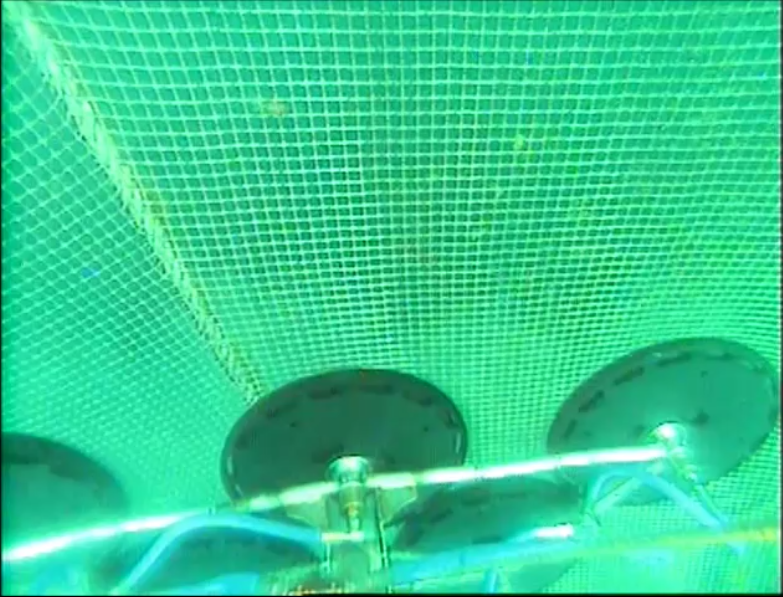
\includegraphics[width=0.9\textwidth]{sintef_not_video_1}
	\caption{Original video provided by SINTEF}
	\label{fig:sintef_not_1}
\end{figure}

\section{SINTEF DVL Test}
This lead to us helping SINTEF out with a doppler velocity log test using a rig for controlling 
the movement of the \todo{not som i garn?}. As a favour for us helping out, we 
got to lend the rig at a later time when our hardware were ready to do a field test. 

During this test, we learned enough ab the rig and operation of it that we should be able to operate 
it ourselves.

\begin{figure}[htbp]
	\centering
	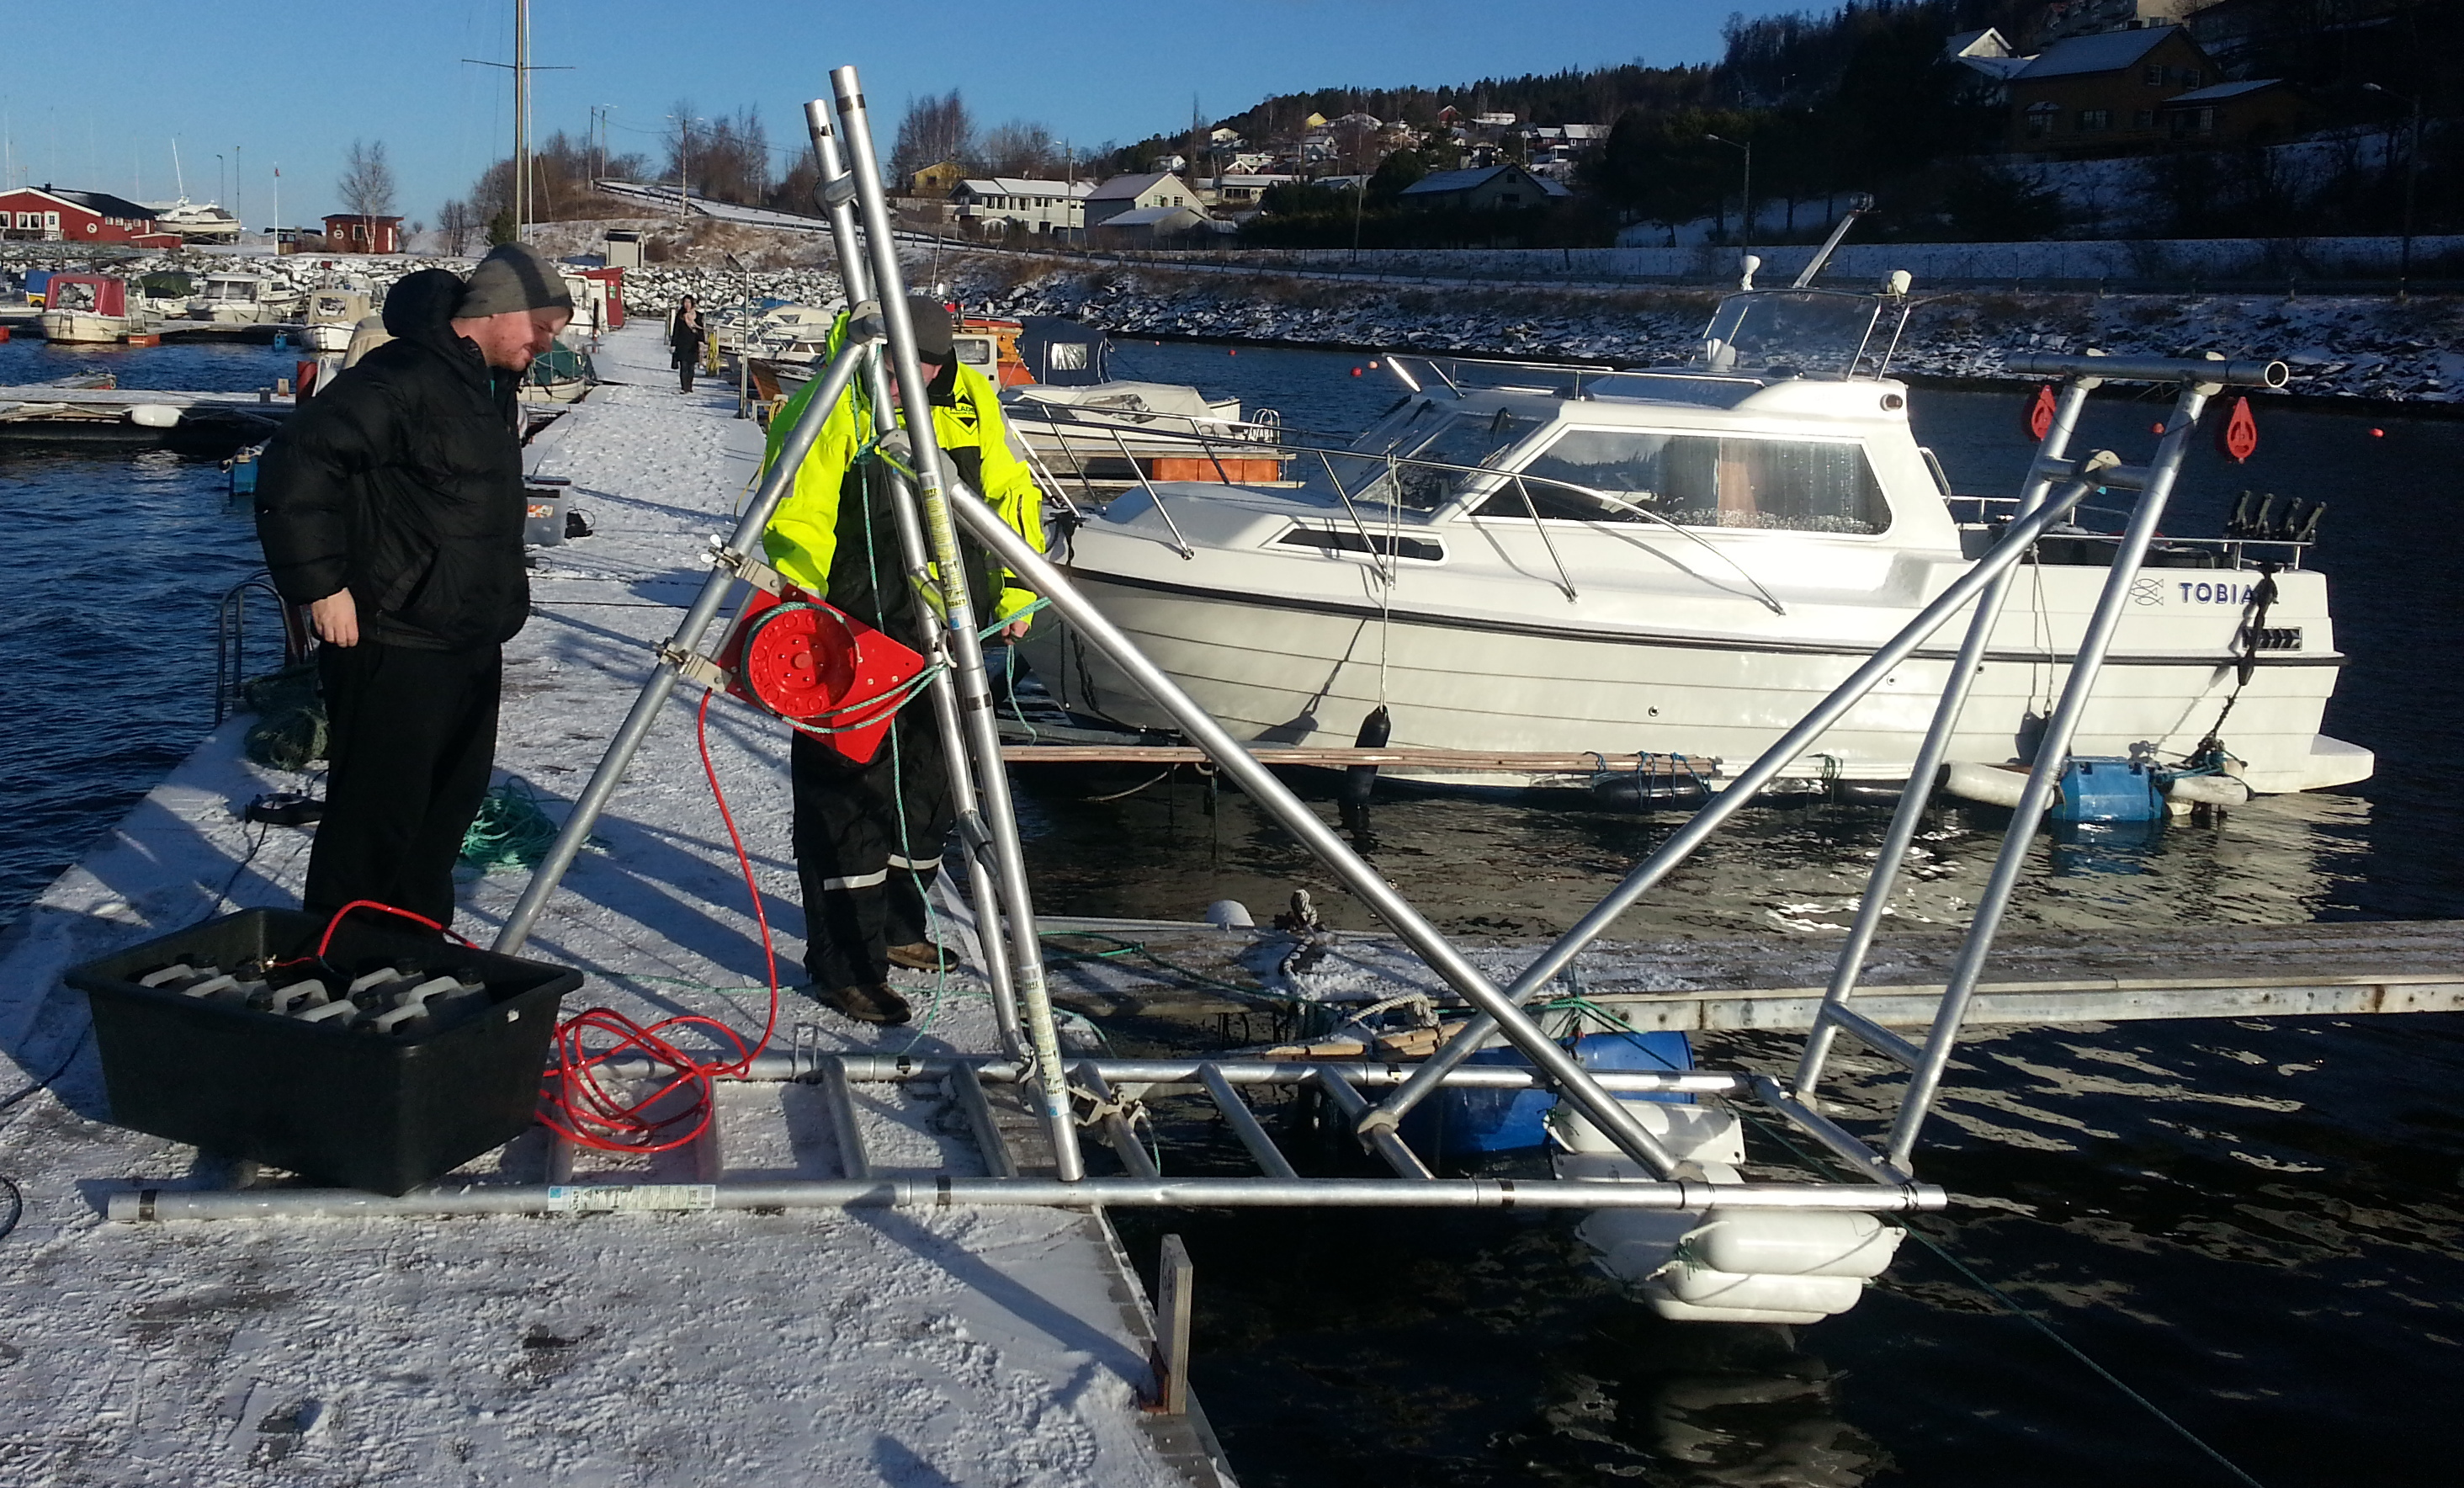
\includegraphics[width=0.9\textwidth]{rig1}
	\caption{Field test for SINTEF using DVL}
	\label{fig:test_dvl}
\end{figure}

\section{HD Video Test}

\begin{figure}[htbp]
	\centering
	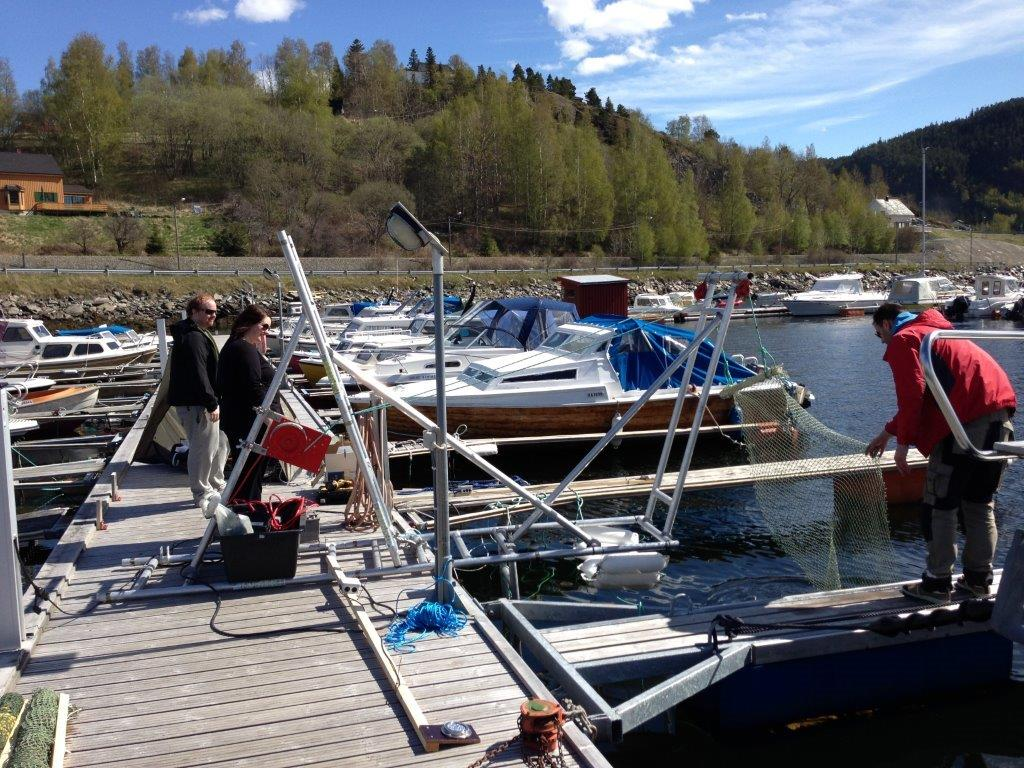
\includegraphics[width=0.9\textwidth]{rig2}
	\caption{Field test}
	\label{fig:test_hd}
\end{figure}

The rig was configured to mimic the approximate distance to the net 
in figure \vref{fig:sintef_not_1}. We were however not able to tilt the camera to 
an angle due to environmental constraint in a anchor chain situated below the camera.
We approximated the distance between the ROV and the net in figure \vref{fig:sintef_not_1} to be 
\SI{1.5}{\metre}. This lead to a the image in \vref{fig:test_hd_referanse}

\begin{figure}[htbp]
	\centering
	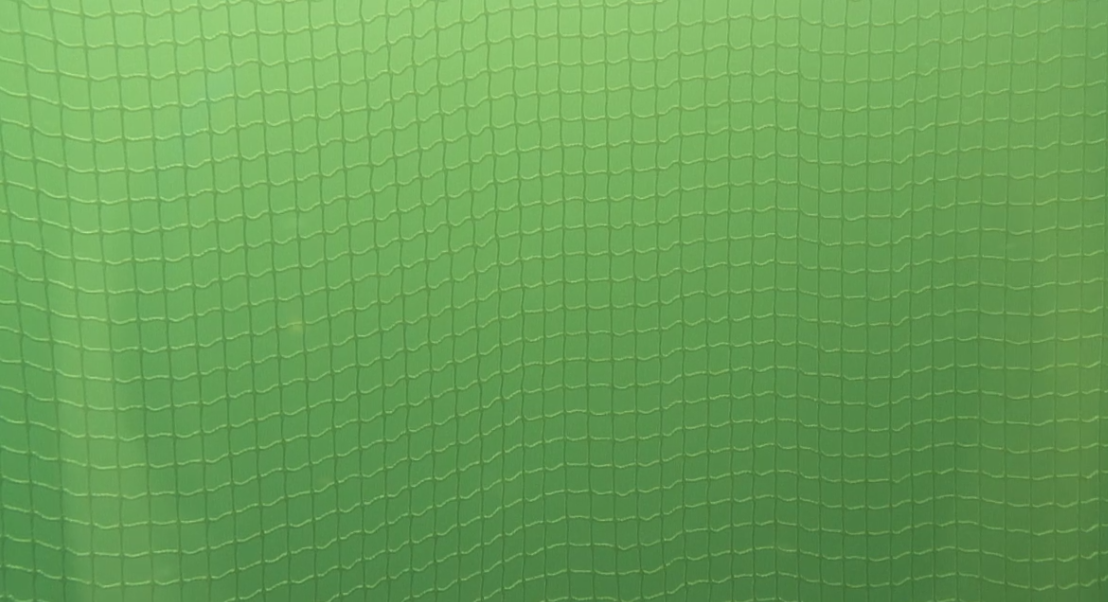
\includegraphics[width=0.9\textwidth]{hd_not_all}
	\caption{View from \SI{1.5}{\metre}}
	\label{fig:test_hd_referanse}
\end{figure}

Comparing image \vref{fig:test_hd_referanse} and \vref{fig:sintef_not_1}, it seems that the 
top row of masks is approximately the same in both images. Due to the tilt of the 
camera in image \ref{fig:sintef_not_1} we get a prominent vanishing point in that image. There 
are also some growing on the net in \ref{fig:sintef_not_1}, which of obvious reasons does not appear 
in \ref{fig:test_hd_referanse}.

\begin{figure}[htbp]
	\centering
	
\includegraphics[width=0.9\textwidth]{hd_not}
	\caption{Field test}
	\label{fig:test_hd_clip}
\end{figure}

\cleardoublepage

\input{impl}
\cleardoublepage


\chapter{Field Tests}\label{ch:field_test}

Computer Vision algorithms can only give as good result as the source videostream that it is 
being fed. After talking a bit to \gls{sintef}, some test videos were provided by them. However, as seen in figure 
\vref{fig:sintef_not_1}, the quality leaves much to be desired. The video provided had a resolution 
of $854 \times 480$ pixels with big black box padding around it. This does not only make 
the video unsuitable for us in a computer vision algorithm, but it also means that the video 
probably is upscaled quite a bit.

Due to the poor nature of the quality of the video it was decided early on that 
a field test was needed, since we were going to use equivalent hardware as to what is available on the \gls{rov}. 

\begin{figure}[htbp]
	\centering
	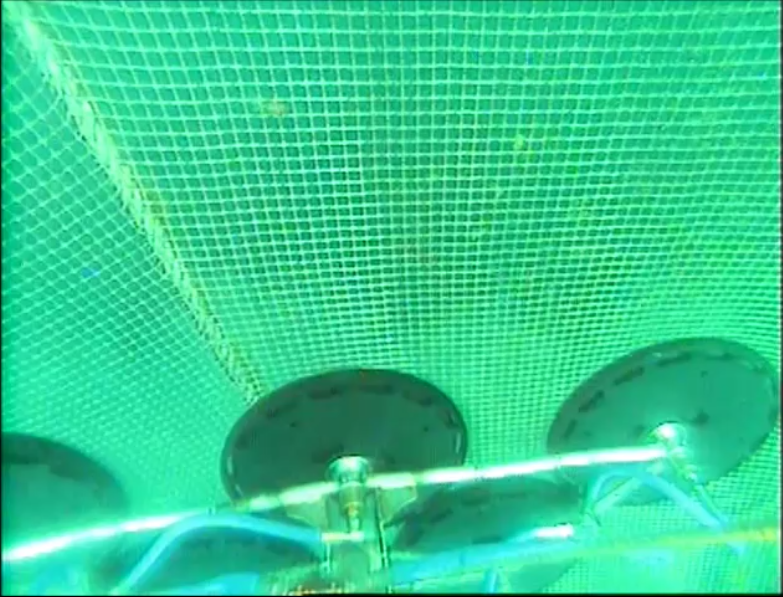
\includegraphics[width=0.9\textwidth]{sintef_not_video_1}
	\caption{Original video provided by \gls{sintef}}
	\label{fig:sintef_not_1}
\end{figure}

\section{SINTEF DVL Test}
This lead to us helping \gls{sintef} out with a \gls{dvl} test using a rig for controlling 
the movement of the net. As a favour for us helping out, we 
got to lend the rig at a later time when our hardware were ready to do a field test. 

During this test, we learned enough about the rig and operation of it that we should be able to operate 
it ourselves.

\begin{figure}[htbp]
	\centering
	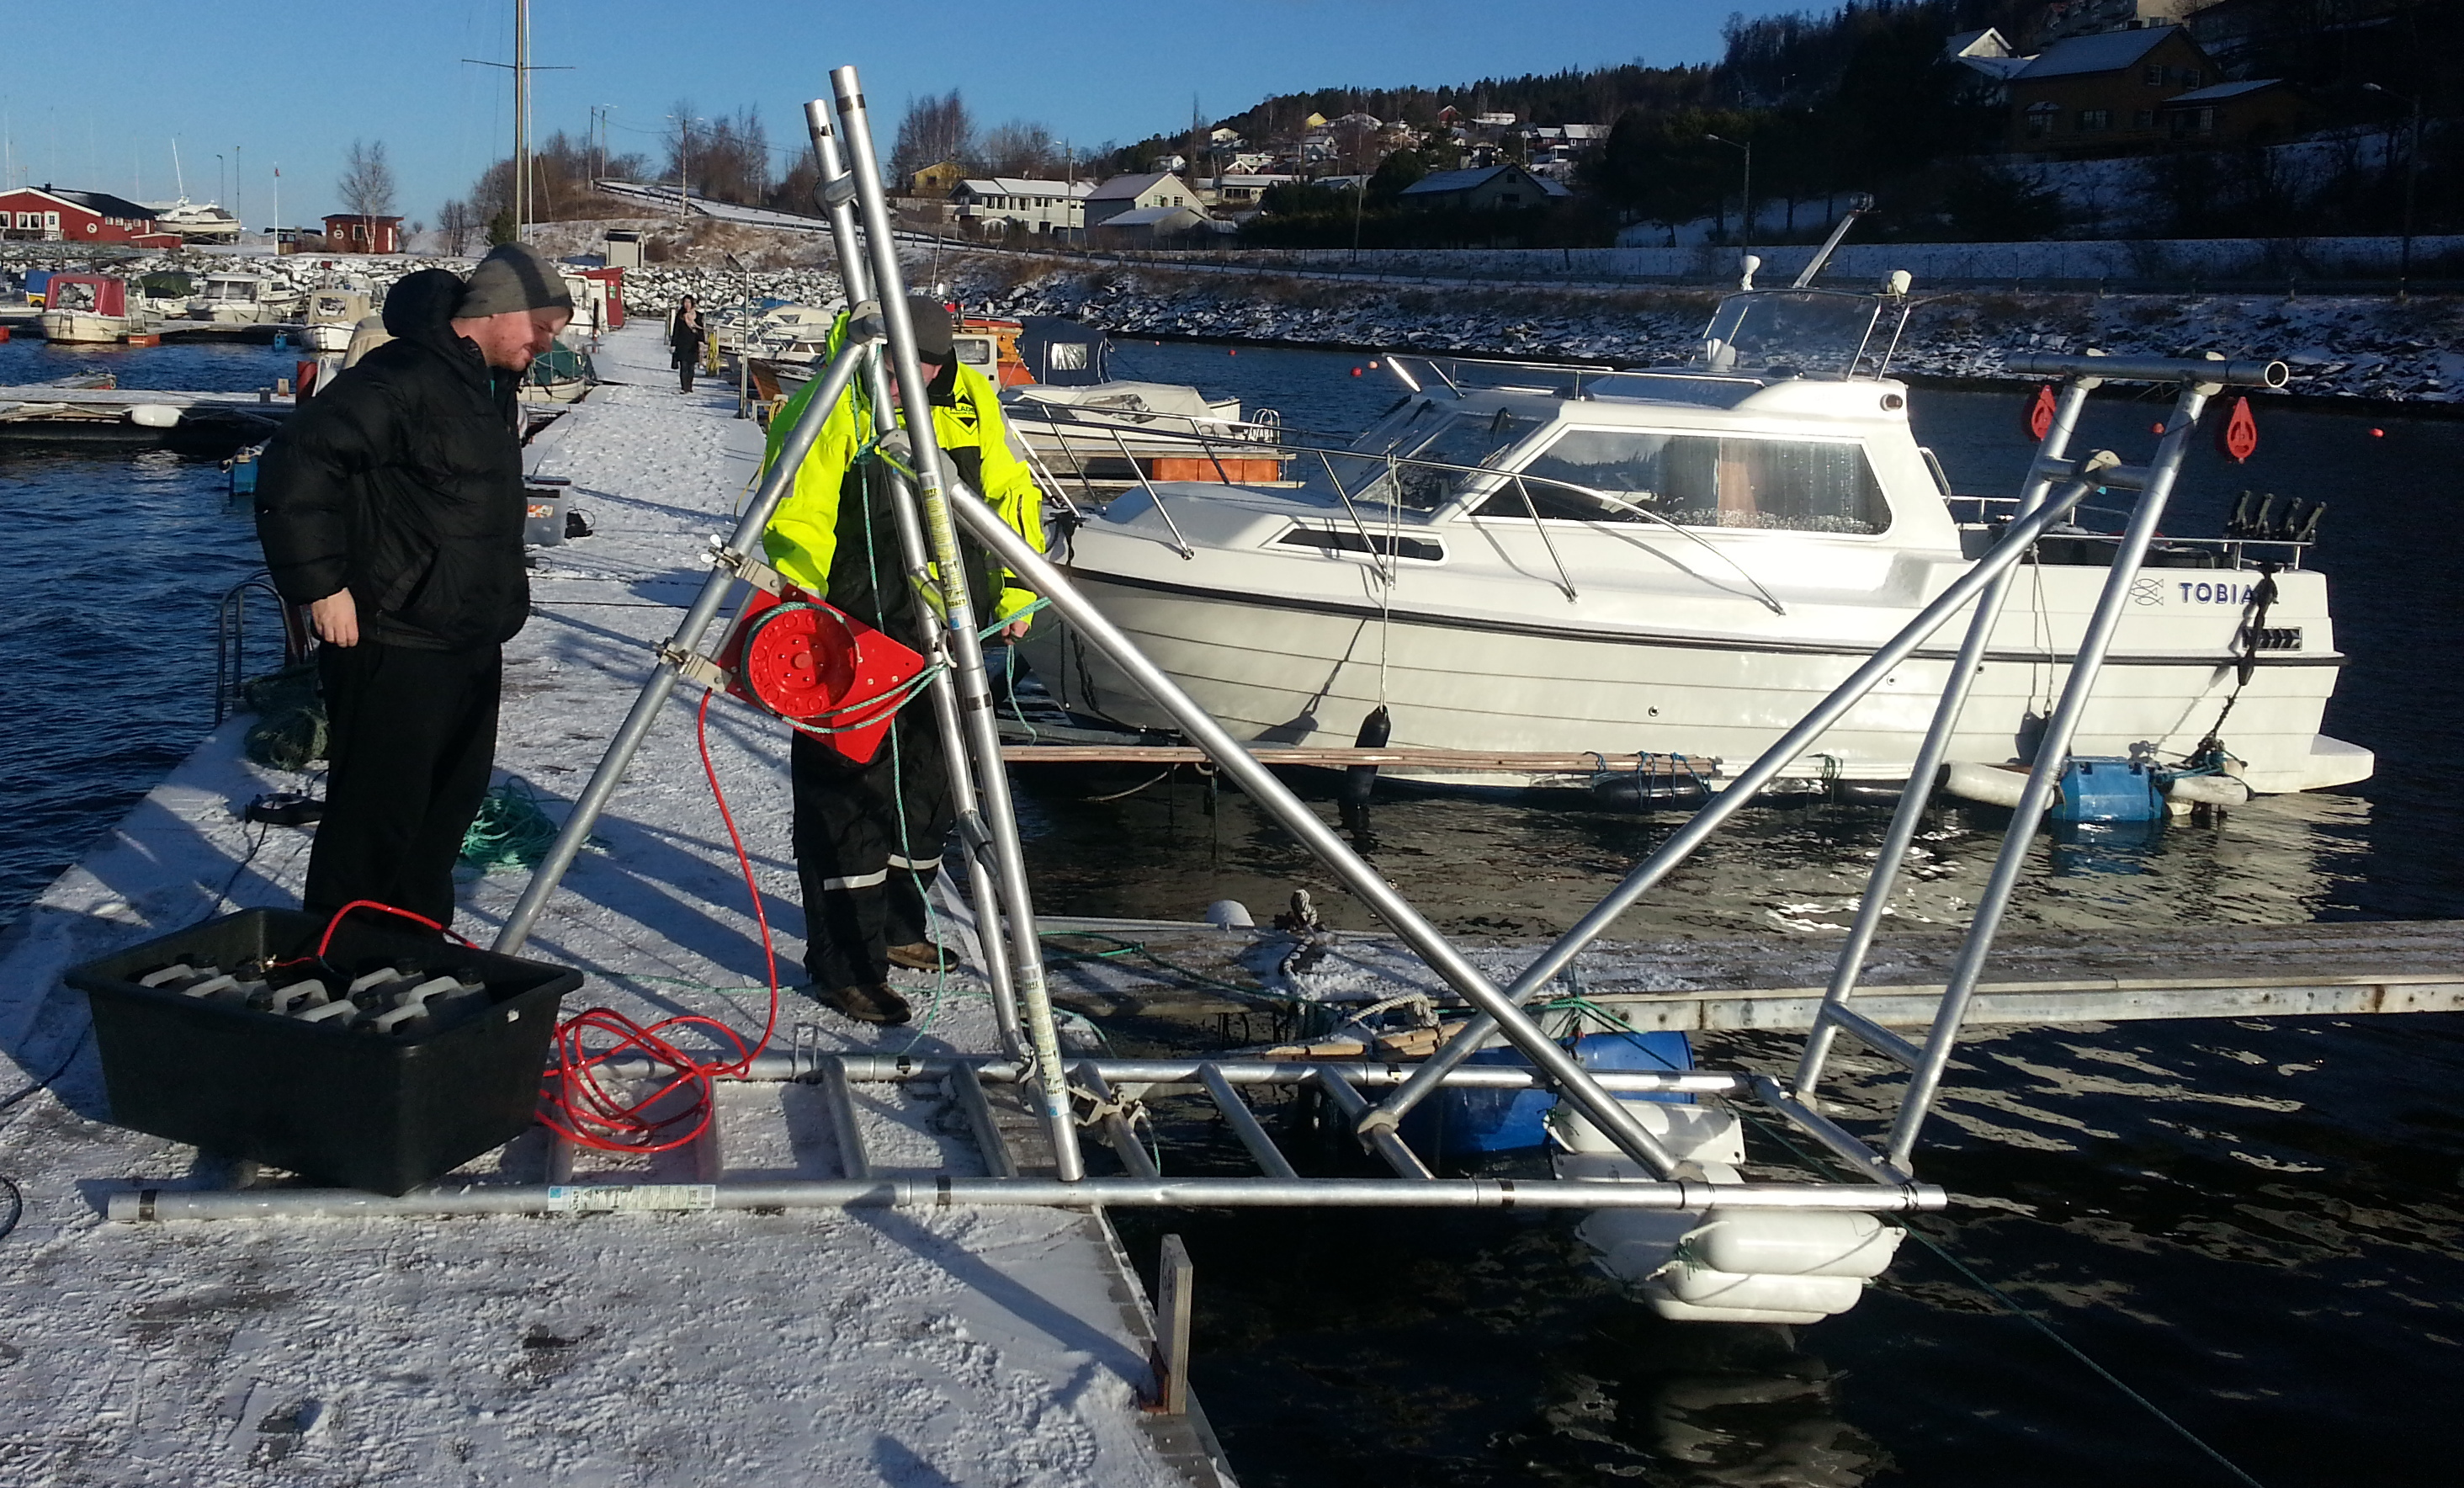
\includegraphics[width=0.9\textwidth]{rig1}
	\caption{Field test for \gls{sintef} using \gls{dvl}}
	\label{fig:test_dvl}
\end{figure}

\section{HD Video Test}

\begin{table}[htbp]
	\centering
	\begin{tabular}{ll}
		\toprule
			Net setup 					& Description  \\
		\midrule
			Reference					& Net in static position. No forced movement. \\
			Reference with movement		& Net lowered in front of the camera. \\
			Circular hole				& Net with a circular cut-out lowered. \\
			Vertical tear				& Net with a narrow vertical tear lowered. \\
			Horizontal tear				& Net with narrow horizontal tear lowered. \\
			L-shaped tear				& Net with horizontal L-shaped tear lowered. \\
			Growth						& Net with imitation growths lowered.\\
			Double sea-cage				& Two nets laid on top of each other.\\
		\bottomrule
	\end{tabular}
	\caption{Test setup, all at \SI{1.5}{\metre}}
	\label{tbl:test_setup}
\end{table}

\begin{figure}[htbp]
    \centering
    \subfloat[Circular Hole]{\label{fig:net_hole}{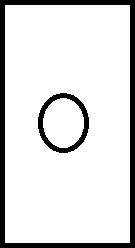
\includegraphics[width=0.3\textwidth]{net_hole}}} \hfill
    \subfloat[Vertical tear]{\label{fig:net_vertical}{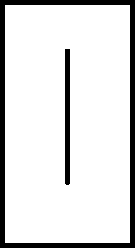
\includegraphics[width=0.3\textwidth]{net_vertical}}} \hfill
    \subfloat[Double net]{\label{fig:net_double}{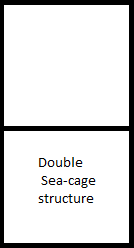
\includegraphics[width=0.3\textwidth]{net_double}}}
    \\
	\subfloat[L-shaped tear]{\label{fig:net_L_tear}{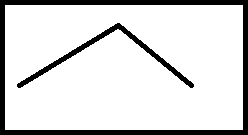
\includegraphics[width=0.45\textwidth]{net_l}}} \hfill
	\subfloat[Horizontal tear]{\label{fig:net_horize}{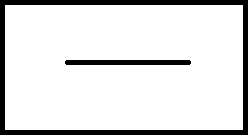
\includegraphics[width=0.45\textwidth]{net_horiz}}}
	\caption{Different net configurations with holes and tears, excluding normal single net. Images collected from \citet{sletta13}.}
	\label{fig:net_configs}
\end{figure}

\begin{figure}[htbp]
	\centering
	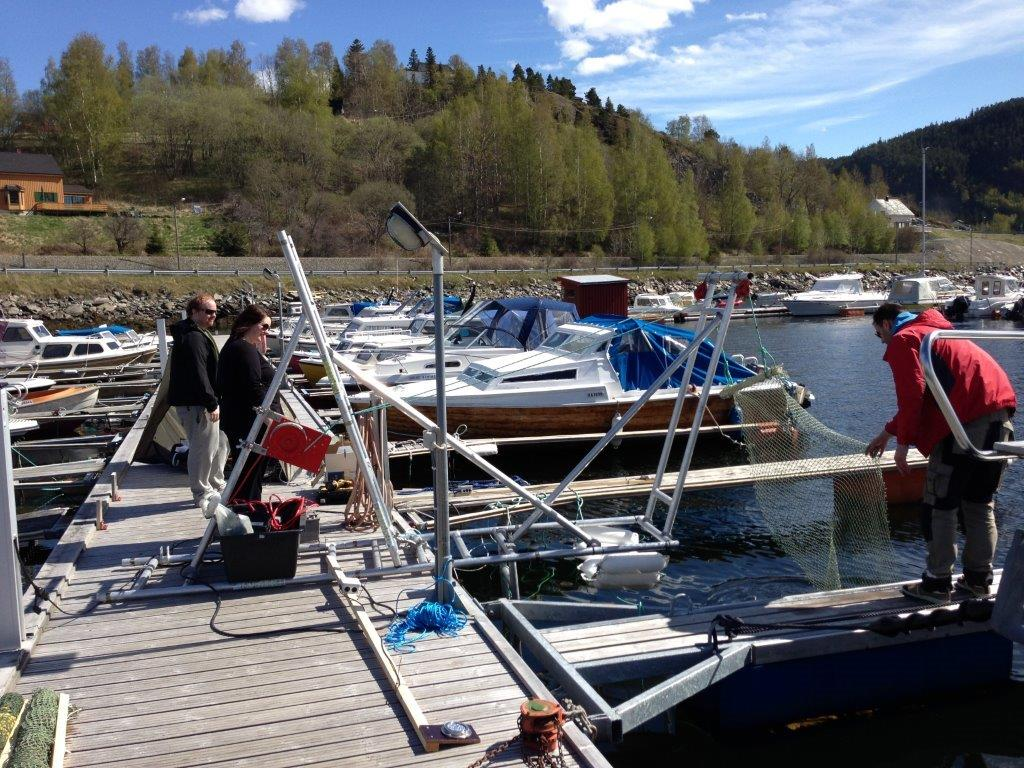
\includegraphics[width=0.9\textwidth]{rig2}
	\caption{Field test on a sunny day in May}
	\label{fig:test_hd}
\end{figure}

The rig was configured to mimic the approximate distance to the net 
in figure \vref{fig:sintef_not_1}. We were however not able to tilt the camera to 
an angle due to environmental constraint in a anchor chain situated below the camera.
We approximated the distance between the ROV and the net in figure \vref{fig:sintef_not_1} to be 
\SI{1.5}{\metre}. This lead to a the image in figure \vref{fig:test_hd_referanse}.

\begin{figure}[htbp]
	\centering
	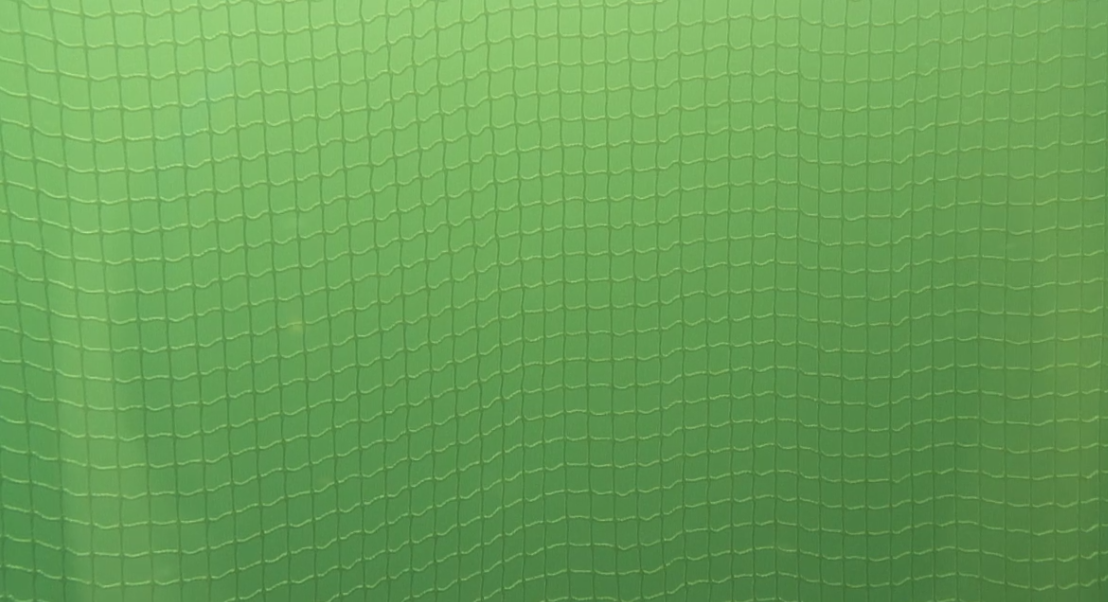
\includegraphics[width=0.9\textwidth]{hd_not_all}
	\caption{View of the net from \SI{1.5}{\metre}. This is the default distance for the rig used.}
	\label{fig:test_hd_referanse}
\end{figure}

Comparing image \vref{fig:test_hd_referanse} and \vref{fig:sintef_not_1}, it seems that the 
top row of masks is approximately the same in both images. Due to the tilt of the 
camera in image \ref{fig:sintef_not_1} we get a prominent vanishing point in that image. There 
are also some growing on the net in figure \ref{fig:sintef_not_1}, which of obvious reasons does not appear 
in figure \ref{fig:test_hd_referanse}.

\begin{figure}[htbp]
	\centering
	
\includegraphics[width=0.9\textwidth]{hd_not}
	\caption{View of masks in the net at \SI{1.5}{\metre}. Digitally zoomed in post processing.}
	\label{fig:test_hd_clip}
\end{figure}

The test was done in accordance with the test patterns described in figure \vref{fig:net_configs}. 
\cleardoublepage

\input{resultat}
\cleardoublepage

\input{diskusjon}
\cleardoublepage

\input{konklusjon}
\cleardoublepage

\input{videre}

\cleardoublepage
\bibliography{bibliography}

\cleardoublepage
\appendix
% !TeX spellcheck = nb_NO

\section{Kondensatorligninger}\label{appendix:cond}
I disse avsnittene er ligningene for parallellplatekondensator, \vref{appendix:parallel}, og 
variabel kapasitanskondensatorer, \vref{appendix:var_cap} gjengitt. 
\subsection{Parallellplatekondensator}\label{appendix:parallel}
Ved å bruke definisjonen av strøm
\begin{equation}
	\frac{\mathrm{d}}{\mathrm{d}t}q(t) = i(t)
	\label{eq:i}
\end{equation}
sammen med ligning \eqref{eq:capactiance} får vi
\begin{equation}
	i(t) = \frac{\mathrm{d}}{\mathrm{d}t}\big(C(t)v(t)\big)
	\label{eq:cap_iv}
\end{equation}

Ligning \eqref{eq:cap_iv} gir en sammenheng mellom strøm gjennom en kondensator og spenning over kondensatoren. 
Det er også tydelig av ligningen at det må legges en varierende spenning 
over kondensatoren for å den skal lede. 

Ved å løse \eqref{eq:cap_iv} med hensyn på \(v(t)\) får vi
\begin{equation}
	v(t) = \frac{1}{C} \int^t_{-\infty}{i(\tau)\,\mathrm{d}\tau}
	\label{eq:cap_v}
\end{equation}
som er standardlikningen for spenningsutvikling over en kondensator ved en variabel strøm, gitt at $C$ er konstant. 

\subsection{Variabel kapasitansligning}\label{appendix:var_cap}
Antagelsen i appendiks \vref{appendix:parallel} er feil, da vi i denne oppgaven 
er ute etter å måle akkurat den \(C\) som varierer med tid, \(C(t)\). 
Om vi bruker definisjonen for \(i(t)\) fra ligning \eqref{eq:i} sammen 
med \eqref{eq:cap_iv}, får vi
\begin{align}
	i(t)  
	&= \frac{\mathrm{d}}{\mathrm{d}t} \big( C(t)v(t) \big)\label{eq:i.3}\\
	&= v(t)\frac{\mathrm{d}}{\mathrm{d}t}C(t) + C(t)\frac{\mathrm{d}}{\mathrm{d}t}v(t) \label{eq:i.4}
\end{align}

Som vi ser av ligning \eqref{eq:i.3} er det umulig å løse dette problemet eksplisitt med tanke på \(C(t)\) 
uten å gjøre antagelse om \(v(t)\) eller \(i(t)\).

Resultatet i ligning \eqref{eq:i.4} er hovedgrunnen til at det ikke er 
mulig å finne absoluttverdier i denne oppgaven.

\section{Enkel oppladningstidmåling}\label{appendix:oppladning}
Som et enkelt eksempel på hvordan er kapasitiv måling kan gjøres, er eksemplet under tatt med. 


En enkel algoritme i pseudokode er også gjengitt. 

\begin{center}
	\begin{circuitikz} \draw
	(0,0) node[anchor=east]{Drivpinne}
		to[short, o-*] (1,0)
		to[R, l=, *-*] (1,2)
	(0,2) node[anchor=east]{Sensorpinne}
		to[short, o-*] (1,2)
		to[C,l=Miljø, *-] (3,2)
		to[short] (3,1) node[ground]{}
	;\end{circuitikz}
\end{center}


%\begin{verbatim}[H]
%\SetAlgoLined
%\KwResult{teller $\propto$ ladetid}
%Initialiser\;
%Set drivpinne høy\;
%\While{sensorpinne ikke høy}{
%	inkrementer teller\;
%}
%\eIf{teller > 0}{
%	resultat = teller\;
%}{
%	feil\;
%}
%\end{verbatim}

Algoritmen over vil gi et tall som er proporsjonalt med antall sykler som er gjort før 
sensorpinnen er kommet opp på logisk 1 ($\approx \frac{V_{dd}}{2}$). Dette er derfor en ''single slope'' måling.

\section{Ladningsoverføring}\label{appendix:mutualcapacitance}
I denne oppgaven er QMatrix\texttrademark fra Atmel valgt som implementasjon av ladningsoverføringsmåling. Atmel utgir dokumentasjon \citet{qtan0079} for de forskjellige teknologiene 
som benyttes og kodebiblioteker for integrasjon i prosjekter.

Den teknologien som er brukt her har sin rot i algoritmen i appendiks \vref{appendix:oppladning}. Det er riktignok en mer komplisert utgave, der hele 
lesesyklusen er vist i appendiks \vref{appendix:mutualcapacitance.4} og i figur \vref{fig:cycle}. En nærmere gjennomgang av 
QMatrix er tilgjengelig i \citet{quantum2006}[QMatrix Technology Whitepaper].

Figur \vref{fig:qmatrix} viser hvordan QMatrix teknologien virker på en pekeflate, som er den primære bruken for QMatrix. 

\begin{figure}[htbp]
	\centering
	\includegraphics[width=0.8\textwidth]{img/qmatrix}
	\caption{QMatrix, hentet fra \citet{quantum2006}}
	\label{fig:qmatrix}
\end{figure}


\clearpage
\subsection{Krets}\label{appendix:mutualcapacitance.circuit}

I figur \vref{fig:chargetransfer} er kretsskjemaet som er brukt i denne oppgaven. Dette skjemaet viser kun 4 punkter, men det er en enkel utvidelse å 
bruke denne kretsen på \(n+m\) punkter som forsøkt vist med subskriptene på linjene.

\begin{figure}[H]
\begin{center}
	\begin{circuitikz}[scale=1.1]
	\draw[dashed,rounded corners] (7.5,9.5) rectangle (5.5,7.5);
	\foreach \x in {8,9} {
		\foreach \y in {6,7} {
			\node[circle,draw] at (\y,\x) {};
		}
	}
	\node[above] at (7.5,9.5) {Membran fra figur \vref{fig:sampl_point}};
	
	\draw
	(0,0) node[anchor=east]{SMP}
		to[short, o-*] (1,0)
		to[R, l=$\text{RYB}_0$] (1,2)
		to[short] (1,3)
		to[short] (0,3)
	(0,3) node[anchor=east]{$\text{YB}_0$}
		to[short, o-*] (1,3)
		to[short] (1,4)
		to[C, l=$\text{CS}_0$] (1,5)
	(0,2) node[anchor=east]{$\text{YB}_m$}
		to[short, o-*] (3,2)
		to[R, l=$\text{RYB}_m$] (3,0)
		to[short] (1,0)
	(3,2) node{}
		to[short] (3,4)
		to[C, l=$\text{CS}_m$] (3,5)
	(0,6) node[anchor=east]{$\text{YA}_m$}
		to[short,o-*] (3,6)
		to[short] (3,5)
	(0,7) node[anchor=east]{$\text{YA}_0$}
		to[short,o-*] (1,7)
		to[short] (1,5)
	(3,6) node{}
		to[R, l=$\text{RY}_m$] (5,6)
		to[short] (7,6)
		to[short] (7,9)
	(1,7) node{} 
		to[short] (3,7)
		to[R, l=$\text{RY}_0$] (5,7)
		to[short] (6,7)
		to[short] (6,9)
	(0,8) node[anchor=east]{$\text{X}_n$}
		to[short, o-*] (3,8)
		to[R, l=$\text{RX}_n$] (5,8)
		to[short] (7,8)
	(0,9) node[anchor=east]{$\text{X}_0$}
			to[short, o-*] (3,9)
			to[R, l=$\text{RX}_0$] (5,9)
			to[short] (7,9)
	;\end{circuitikz}
\end{center}
\caption{Ladningsoverføringskrets}
\label{fig:chargetransfer}
\end{figure}

\pagebreak
Forkortelser og linjer brukt i figur \vref{fig:chargetransfer} er beskrevet under.

\begin{description}
	\item[$\text{X}_n$] Drivlinjene. Kobles til en I/O port.
	\item[$\text{YA}_m$] I/O Porter. Her vil spenningen over $\text{CS}_m$ legge seg. Brukes for å lade ut $\text{CS}_m$.
	\item[$\text{YB}_m$] ADC porter. Måler utviklingen av oppladningen over $\text{CS}_m$.
	\item[SMP] Generel I/O port. Pulser tilbake over $\text{CS}_m$. Dette setter opp en negativ spenning som driver $\text{CS}_m$ tilbake mot 0
	\item[$\text{RYB}_m$] Pull-down resistor 
	\item[$\text{CS}_m$] Samplingkondensator. Lades opp av $\text{X}_m$
\end{description}

Den kretsen som er skissert i figur \vref{fig:chargetransfer} vil ha flere ekvivalenter ettersom hvilken del av oppladningssykelen som kretsen
er i. Disse ekvivalentene er gjennomgått i appendiks \vref{appendix:mutualcapacitance.1}, \vref{appendix:mutualcapacitance.2} og \vref{appendix:mutualcapacitance.3}.

\vfill

\pagebreak
\subsection{Ekvivalenskrets under oppladning}\label{appendix:mutualcapacitance.1}
\begin{figure}[H]
\begin{center}
	\begin{circuitikz}[scale=1.3]
	\draw[dashed,rounded corners] (7.5,9.5) rectangle (5.5,7.5);
		\foreach \x in {8,9} {
			\foreach \y in {6,7} {
				\node[circle,draw] at (\y,\x) {};
			}
		}
		\node[above] at (7.5,9.5) {Membran fra figur \vref{fig:sampl_point}};
		
	
	\draw
	(0,0) node[anchor=east]{SMP}
		to[short, o-*] (1,0)
		to[R, l=$\text{RYB}_0$] (1,2)
		to[short] (1,3)
		to[short] (1,4)
		to[C, l=$\text{CS}_0$] (1,5)
	(0,-1) node[ground]{}
		to[short](0,0)
	%(0,3) node[anchor=east]{$\text{YB}_0$}
	%	to[short, o-*] (1,3)
	%	to[short] (1,4)
	%	to[C, l=$\text{CS}_0$] (1,5)
	%(0,2) node[anchor=east]{$\text{YB}_m$}
	%	to[short, o-*] (3,2)
	%	to[R, l=$\text{RYB}_m$] (3,0)
	%	to[short] (1,0)
	(3,2) node{}
		to[R, l=$\text{RYB}_m$] (3,0)
		to[short] (1,0)
	(3,2) node{}
		to[short] (3,4)
		to[C, l=$\text{CS}_m$] (3,5)
	%(0,6) node[anchor=east]{$\text{YA}_m$}
	%	to[short,o-*] (3,6)
	%	to[short] (3,5)
	%(0,7) node[anchor=east]{$\text{YA}_0$}
	%	to[short,o-*] (1,7)
	%	to[short] (1,5)
	(3,6) node{} 
		to[short] (3,5)
	(1,7) node{}
		to[short] (1,5)
		
	(3,6) node{}
		to[R, l=$\text{RY}_m$] (5,6)
		to[short] (7,6)
		to[short] (7,9)
	(1,7) node{} 
		to[short] (3,7)
		to[R, l=$\text{RY}_0$] (5,7)
		to[short] (6,7)
		to[short] (6,9)
	(0,8) node[anchor=east]{$\text{X}_n$}
		to[short, o-*] (3,8)
		to[R, l=$\text{RX}_n$] (5,8)
		to[short] (7,8)
	(0,9) node[anchor=east]{$\text{X}_0$}
			to[short, o-*] (3,9)
			to[R, l=$\text{RX}_0$] (5,9)
			to[short] (7,9)
	;\end{circuitikz}
\end{center}
\caption{Ekvivalenskrets under oppladning}
\label{fig:chargetransfer_in}
\end{figure}

\pagebreak
\subsection{Ekvivalenskrets under motladning}\label{appendix:mutualcapacitance.2}
\begin{figure}[H]
\begin{center}
	\begin{circuitikz}[scale=1.8] \draw
	(0,5.5) node[ground]{}
		to[short] (0,6)
		to[short] (0,7)
	(0,0) node[anchor=east]{SMP}
		to[short, o-*] (1,0)
		to[R, l=$\text{RYB}_0$] (1,2)
		to[short] (1,3)
		to[short] (1,4)
		to[C, l=$\text{CS}_0$] (1,5)
	(0,3) node[anchor=east]{$\text{YB}_0$}
		to[short, o-*] (1,3)
		to[short] (1,4)
	(0,2) node[anchor=east]{$\text{YB}_m$}
		to[short, o-*] (3,2) 
	(3,2) node{}
		to[R, l=$\text{RYB}_m$] (3,0)
		to[short] (1,0)
	(3,2) node{}
		to[short] (3,4)
		to[C, l=$\text{CS}_m$] (3,5)
	(0,6) node[anchor=east]{$\text{YA}_m$}
		to[buffer] (3,6)
		to[short] (3,5)
	(0,7) node[anchor=east]{$\text{YA}_0$}
		to[short,o-*] (1,7)
		to[short] (1,5)
	(3,6) node{} 
		to[short] (3,5)
	(1,7) node{}
		to[short] (1,5)
		
	%(3,6) node{}
	%	to[R, l=$\text{RY}_m$] (5,6)
	%	to[short] (7,6)
	%	to[short] (7,9)
	%(1,7) node{} 
	%	to[short] (3,7)
	%	to[R, l=$\text{RY}_0$] (5,7)
	%	to[short] (6,7)
	%	to[short] (6,9)
	%(0,8) node[anchor=east]{$\text{X}_n$}
	%	to[short, o-*] (3,8)
	%	to[R, l=$\text{RX}_n$] (5,8)
	%	to[short] (7,8)
	%(0,9) node[anchor=east]{$\text{X}_0$}
	%		to[short, o-*] (3,9)
	%		to[R, l=$\text{RX}_0$] (5,9)
	%		to[short] (7,9)
	;\end{circuitikz}
\end{center}
\caption{Ekvivalenskrets under motladning}
\label{fig:chargetransfer_out}
\end{figure}



\pagebreak
\subsection{Ekvivalenskrets under utladning}\label{appendix:mutualcapacitance.3}
\begin{figure}[H]
\begin{center}
	\begin{circuitikz}[scale=1.5] \draw
	(0,5.5) node[ground]{}
		to[short] (0,6)
		to[short] (0,7)
	(0,0) node[anchor=east]{SMP}
		to[short, o-*] (1,0)
		to[R, l=$\text{RYB}_0$] (1,2)
		to[short] (1,3)
		to[short] (1,4)
		to[C, l=$\text{CS}_0$] (1,5)
	(0,3) node[anchor=east]{$\text{YB}_0$}
		to[short, o-*] (1,3)
		to[short] (1,4)
	(0,2) node[anchor=east]{$\text{YB}_m$}
		to[short, o-*] (3,2) 
	(3,2) node{}
		to[R, l=$\text{RYB}_m$] (3,0)
		to[short] (1,0)
	(3,2) node{}
		to[short] (3,4)
		to[C, l=$\text{CS}_m$] (3,5)
	(0,6) node[anchor=east]{$\text{YA}_m$}
		to[buffer] (3,6)
		to[short] (3,5)
	(0,7) node[anchor=east]{$\text{YA}_0$}
		to[short,o-*] (1,7)
		to[short] (1,5)
	(3,6) node{} 
		to[short] (3,5)
	(1,7) node{}
		to[short] (1,5)
	(0,-1) node[ground]{}
		to[short](0,0)
	%(3,6) node{}
	%	to[R, l=$\text{RY}_m$] (5,6)
	%	to[short] (7,6)
	%	to[short] (7,9)
	%(1,7) node{} 
	%	to[short] (3,7)
	%	to[R, l=$\text{RY}_0$] (5,7)
	%	to[short] (6,7)
	%	to[short] (6,9)
	%(0,8) node[anchor=east]{$\text{X}_n$}
	%	to[short, o-*] (3,8)
	%	to[R, l=$\text{RX}_n$] (5,8)
	%	to[short] (7,8)
	%(0,9) node[anchor=east]{$\text{X}_0$}
	%		to[short, o-*] (3,9)
	%		to[R, l=$\text{RX}_0$] (5,9)
	%		to[short] (7,9)
	;\end{circuitikz}
\end{center}
\caption{Ekvivalenskrets under utladning}
\label{fig:chargetransfer_reset}
\end{figure}

\pagebreak
\section{Ladesykel over \texorpdfstring{$\text{CS}_m$}{Cs}}\label{appendix:mutualcapacitance.4}


\begin{sidewaysfigure}
\begin{figure}[H]
\begin{center}
\begin{tikzpicture}[xscale=15]
	%\draw[help lines,step=0.1] (0,-8) grid (1,7);
	\draw [->, help lines] (0,-7) -- (0,6);
	\draw [->, help lines] (0,0) -- (1,0);
	\draw[rounded corners] (0,0) -- (0.04,1) -- (0.08,1) -- (0.12,2) -- (0.16,2) -- (0.20,3) -- (0.24,3) -- (0.28,4) -- (0.32,4) -- (0.36,5) -- (0.4,5) -- (0.44,4) -- (0.48,4) -- (0.52,3) -- (0.56,3) -- 
		(0.6,2) -- (0.64,2) -- (0.68,1) -- (0.72,1) -- (0.76,0) -- (0.80,0) -- (0.84,-1) -- (0.88,-1) -- (0.92,-2) -- (0.96,-2) -- (1,0);
	\draw[thin,dashed] (0.38,-7) -- (0.38,6);
	\node[above] at (0.36,6) {1. fase ferdig};
	\node[right] at (0.4,5) {Start utladning};
	\draw[thin,dashed] (0.78,-7) -- (0.78,6);
	\node[above] at (0.76,6) {2. fase ferdig};
	\draw[thin,dashed] (0.94,-7) -- (0.94,6);
	\node[above,align=center] at (0.94,6) {3. fase ferdig};
	
	\node[left] at (0,0) {$V_{\text{CS}_m}$};
	\node[left] at (0,-3) {$\text{X}_n$};
	\node[left] at (0,-5) {SMP};
	\node[left] at (0,-7) {$\text{YA}_m$};
	
	\draw[<->] (0.15,3) -- (0.15,4);
	\draw[dashed] (0.2,3) -- (0.15,3);
	\draw[dashed] (0.29,4) -- (0.15,4);
	\node[left] at (0.15,3.5) {$v_\delta$};
	
	\draw[<->]  (0.52,-2.5) -- (0.56,-2.5);
	\draw[dashed] (0.52,-4) -- (0.52,-2.5);
	\draw[dashed] (0.56,-4) -- (0.56,-2.5);
	\node[above] at (0.54,-2.5) {ADC};
	
	\draw [->, help lines] (0,-3) -- (1,-3);
	\draw (0,-2) -- (0.04,-2) -- (0.04,-3) -- (0.08,-3) -- (0.08,-2) -- (0.12,-2) -- (0.12,-3) -- (0.16,-3) -- (0.16,-2) -- (0.2,-2) -- (0.2,-3) -- (0.24,-3) -- (0.24,-2) -- (0.28,-2) -- (0.28,-3) -- 
		(0.32,-3) -- (0.32,-2) -- (0.36,-2) -- (0.36,-3);
	
	\draw [->, help lines] (0,-5) -- (1,-5);
	\draw (0.4,-5) -- (0.4,-4) -- (0.44,-4) -- (0.44,-5) -- (0.48,-5) -- (0.48,-4) -- (0.52,-4) -- (0.52,-5) -- (0.56,-5) -- (0.56,-4) -- (0.60,-4) -- (0.60,-5) -- (0.64,-5) -- (0.64,-4) -- (0.68,-4) -- 
		(0.68,-5) -- (0.72,-5) -- (0.72, -4) -- (0.76,-4) -- (0.76,-5) -- (0.80,-5) -- (0.80,-4) -- (0.84,-4) -- (0.84,-5) -- (0.88,-5) -- (0.88,-4) -- (0.92,-4) -- (0.92,-5);
		
	\draw [->, help lines] (0,-7) -- (1,-7);
\end{tikzpicture}
\end{center}
\caption{Skjematisk tegning av ladesykel over $\text{CS}_m$}
\label{fig:cycle}
\end{figure}
\end{sidewaysfigure}

Figur \vref{fig:cycle} gjengir en full lesesyklus for oppsettet. 

\subsection{Fase 1}
I den første delen av figur \vref{fig:cycle} fungerer kretsen som vist i figur \vref{fig:chargetransfer_in} i appendiks \vref{appendix:mutualcapacitance.1}.

Her blir \(\text{X}_n\) brukt til å øke spenningen over \(\text{CS}_m\). Avhengig av avstanden mellom elektrodene så vil \(v_\delta\) bli større eller mindre, og 
vil dermed endre høyden på pyramiden, da det er et fast antall pulser på \(\text{X}_n\) i denne delen.

\subsection{Fase 2}\label{appendix:down}
I den andre delen av figur \vref{fig:cycle} fungerer kretsen som vist i figur \vref{fig:chargetransfer_out} i appendiks \vref{appendix:mutualcapacitance.2}. 

Her blir porten merket SMP  brukt til å lade alle kondensatorene ut. Mellom hver puls på SMP brukes ADC funksjonaliteten i mikrokontrolleren til å 
måle spenningen som ligger over alle kondensatorene. Om denne går under nullpotensialet vil antall pulser som er brukt i denne delen være et mål 
på hvor mye spenning som ble lagt over kondensatoren. Dette er en klassisk dobbelthelningsmåling\footnote{dual-slope}, som brukes da målingene blir mindre støyutsatt, og 
fysiske endringer med kondensatorene kan motvirkes til en viss grad.

\subsection{Fase 3}
I den tredje delen av figur \vref{fig:cycle} fungerer kretsen som vist i figur \vref{fig:chargetransfer_reset} i appendiks \vref{appendix:mutualcapacitance.3}.

Etter nedladningsdelen i \vref{appendix:down} vil mest sannsynlig flere av kondensatorene ha en negativ spenning, og de må derfor settes tilbake 
til et kjent nullpotensiale slik at oppladningssyklusen begynner fra et kjent spenning.

\end{document}
